\section{Procedimento \& Analisi Dati}

Nell'ottica geometrica si usano le leggi del costruttore di lenti e dei punti coniugati.
Tali leggi si basano sulle ipotesi di raggi parassiali e lenti sottili, che dobbiamo quindi supporre verificate
nel nostro apparato sperimentale. Una parte dell'esperienza, quella relativa alle due tipologie di aberrazione, è dedicata alla misura dei limiti di tali approssimazioni.

\begin{figure}[b!]
	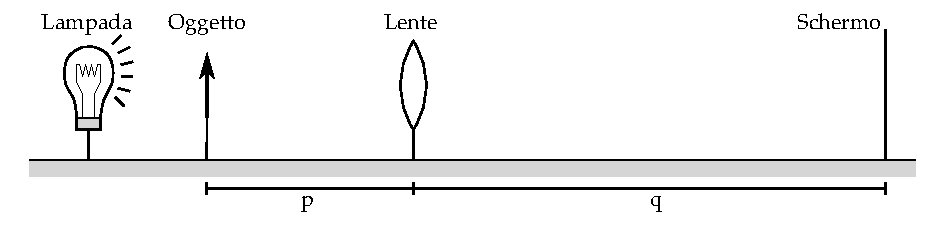
\includegraphics[width=16cm]{drawing.pdf}
    \caption{Schema dell'apparato sperimentale usato per la misura del fuoco della lente convergente.}
    \label{fig:conv}
\end{figure}

\subsection{Fuoco della lente convergente}

Per non appesantire la lettura, nel seguito indicheremo con queste lettere le seguenti quantità (si veda la Figura \ref{fig:conv}):

\begin{equation*}
	p \,=\, \text{distanza tra il centro della lente e la posizione dell'oggetto}
\end{equation*}
\begin{equation*}
	q \,=\, \text{distanza tra il centro della lente e la posizione dell'immagine}
\end{equation*}
\begin{equation*}
	f \,=\, \text{fuoco della lente analizzata}
\end{equation*}
\begin{equation*}
	h \ped{imm} \,=\, \text{altezza dell'immagine sullo schermo}
\end{equation*}
%\begin{equation}
%	\text{Legge dei punti coniugati:} \qquad \frac{1}{f} \,=\, \frac{1}{p} + \frac{1}{q}
%	\label{eq:coniugati}
%\end{equation}
%\begin{equation}
%	\text{Legge del costruttore di lenti:} \qquad \frac{1}{f} \,=\, (n-1)\left(\frac{1}{R\ped{1}}-\frac{1}{R\ped{2}}\right)
%	\label{eq:costruttore}
%\end{equation}


Come primo obiettivo ci siamo posti di calcolare il fuoco e l'ingrandimento della lente convergente per diversi valori di $p$ e $q$. Abbiamo quindi misurato dodici valori di $q$ e di $h\ped{imm}$ al variare di $p$.
Questo è stato fatto tenendo ferma la sorgente luminosa e allontanando la lente divergente in modo tale da aumentare $p$, mettendo a fuoco di volta in volta l'immagine sullo schermo. %<-- questa frase ha sostituito questa -->%Questo è stato fatto tenendo ferma la sorgente luminosa, incrementando di volta in volta la distanza tra la lente e la sorgente luminosa e mettendo a fuoco l'immagine sullo schermo.
Una volta definita la distanza oggetto lente $p$, si è poi misurata la distanza lente-schermo $q$ e la dimensione $h\ped{imm}$ dell'immagine proiettata sullo schermo. Le misure di distanza sono state eseguite con il metro a nastro prestando attenzione a minimizzare l'inclinazione del metro rispetto all'asse ottico. Inoltre la lettura è stata eseguita nel centro della lente. Le misure di dimensione dell'immagine sono invece state eseguite con il calibro ventesimale.

Ovviamente, la distanza oggetto-lente è stata mantenuta maggiore della distanza focale ($p > f$). In caso contrario si avrebbe infatti un immagine virtuale e sarebbe impossibile mettere a fuoco l'immagine sullo schermo.

E' importante sottolineare che nel caso in cui l'immagine si è formata ad una grande distanza dalla lente, riuscire a metterla a fuoco non è stato semplice a causa dell'effetto di profondità di campo. Abbiamo deciso quindi di prendere due misure $q_1$ e $q_2$, con la seguente procedura: quando l'immagine era circa a fuoco, abbiamo mosso lo schermo in avanti e in dietro in modo da avere l'immagine leggermente fuori fuoco in entrambe le direzioni e abbiamo quindi annotato le due distanze. Ciò ci è stato utile in quanto per l'occhio umano è più facile vedere quando un oggetto è fuori fuoco rispetto al fuoco perfetto. Facendo la media di questi due valori abbiamo ottenuto un valore di $q$ %probabilmente? mah...
più preciso rispetto alla misura diretta.

Una volta ottenuti i valori  di $p$ e $q$, abbiamo calcolato per ognuno il relativo valore di $f$ utilizzando la legge dei punti coniugati:
\begin{equation}
	\frac{1}{f} \,=\, \frac{1}{p} + \frac{1}{q}
	\label{eq:coniugati}
\end{equation}

Quindi è stata calcolata la media aritmetica dei valori, con la quale abbiamo ottenuto il seguente valore della focale:
\begin{equation}
    f \ped{conv} \,=\, 24.0 \pm 0.6 \; \si{\centi\metre}
\end{equation}

Vogliamo inoltre ricavare il valore della magnificazione per ogni coppia $p$ e $q$.
%io salterei questa frase -->%Ricordiamo che la magnificazione è il rapporto tra le dimensioni dell'immagine ottenuta ($h \ped{imm}$) rispetto alle dimensioni reali dell'oggetto ($h$).
Sapendo che la dimensione dell'oggetto era $h = \SI{9}{\milli\metre}$, dato che consideriamo privo di errore, l'ingrandimento vale: 

\begin{equation}
    m\ped{h} \,=\, \frac{h \ped{imm}}{h}
\end{equation}

Infine per avere una verifica della correttezza dei dati registrati, abbiamo messo a confronto il valore della magnificazione trovato empiricamente con quello che si può ricavare dalla seguente relazione:

\begin{equation}
    m\ped{pq} \,=\, \frac{q}{p}
\end{equation}

%Tabella $m_1$, $m_2$, p, q, $h_{imm}$ e incertezze. Forse f?

%\begin{center}
\begin{table}
    \centering
    \small
    \begin{tabular}{c c c c c c}
        \toprule
        $p \; [\si{\centi\metre}]$ & $q \; [\si{\centi\metre}]$ & $f \; [\si{\centi\metre}]$ &
        $h\ped{imm} \; [\si{\centi\metre}]$ & $m\ped{h}$ & $m\ped{pq}$ \\
        \midrule
        28.8 $\pm$ 0.05 & 149.35 $\pm$ 0.05 & 24 $\pm$ 1 & 4.59 $\pm$ 0.01 & 5.100 $\pm$ 0.002  & 5.19 $\pm$ 0.01 \\
		30.8 $\pm$ 0.05 & 111.75 $\pm$ 0.05 & 24 $\pm$ 1 & 3.22 $\pm$ 0.01 & 3.583 $\pm$ 0.00 & 3.628 $\pm$ 0.0063 \\
		32.8 $\pm$ 0.05 & 91.85 $\pm$ 0.05 & 24 $\pm$ 1 & 2.49 $\pm$ 0.01 & 2.767 $\pm$ 0.004& 2.800 $\pm$ 0.005  \\
		34.9 $\pm$ 0.05 & 77.60 $\pm$ 0.05 & 24 $\pm$ 1 & 1.85 $\pm$ 0.01 & 2.056 $\pm$ 0.005& 2.223 $\pm$ 0.003  \\
		36.9 $\pm$ 0.05 & 69.60 $\pm$ 0.05 & 24 $\pm$ 1 & 1.69 $\pm$ 0.01 & 1.878 $\pm$ 0.006& 1.886 $\pm$ 0.003  \\
		38.8 $\pm$ 0.05 & 63.00 $\pm$ 0.05 & 24 $\pm$ 1 & 1.44 $\pm$ 0.01 & 1.600 $\pm$ 0.007& 1.624 $\pm$ 0.002  \\
		40.8 $\pm$ 0.05 & 58.50 $\pm$ 0.05 & 24 $\pm$ 1 & 1.28 $\pm$ 0.01 & 1.422 $\pm$ 0.008& 1.434 $\pm$ 0.002  \\
		42.8 $\pm$ 0.05 & 54.90 $\pm$ 0.05 & 24 $\pm$ 1	& 1.13 $\pm$ 0.01 & 1.26 $\pm$ 0.01  & 1.283 $\pm$ 0.002  \\
		44.8 $\pm$ 0.05 & 51.70 $\pm$ 0.05 & 24 $\pm$ 1 & 0.99 $\pm$ 0.01 & 1.10 $\pm$ 0.01  & 1.154 $\pm$ 0.002  \\
		46.9 $\pm$ 0.05 & 49.20 $\pm$ 0.05 & 24 $\pm$ 1 & 0.91 $\pm$ 0.01 & 1.02 $\pm$ 0.01  & 1.049 $\pm$ 0.002  \\
		48.9 $\pm$ 0.05 & 47.40 $\pm$ 0.05 & 24 $\pm$ 1 & 0.85 $\pm$ 0.01 & 0.94 $\pm$ 0.01  & 0.969 $\pm$ 0.001  \\
		50.9 $\pm$ 0.05 & 45.40 $\pm$ 0.05 & 23 $\pm$ 1 & 0.78 $\pm$ 0.01 & 0.87 $\pm$ 0.01  & 0.892 $\pm$ 0.001  \\
        \bottomrule
    \end{tabular}
    \caption{La tabella riporta i dati misurati e i risultati dei calcoli eseguiti.}
    \label{tab:conv}
\end{table}
%\end{center}

% in realtà non so se vuole tutti sti dati, però secondo me è meglio metterceli, perché
% in una relazione scientifica si mettono sempre tutti i dati per permettere agli altri di controllare eventuali
% errori. Comunque almeno m_1 e m_2... FRAPA X BUZZ
%vediamo quanto occupano dai... intanto io li ho messi BUZZ X FRAPA
% PS: forse sarebbe meglio invertire le colonne h_imm e m_1 BUZZ X FRAPA

Come si può osservare dai dati nella Tabella \ref{tab:conv}, i due valori della magnificazione ricavati con i diversi procedimenti
non sono sempre compatibili. In molti casi essi sono compatibili entro un sigma, mentre in altri casi sono anche molto lontani. Questo
è probabilmente imputabile alle misure di fuoco, piuttosto che alle misure di dimensione dell'immagine.
% X BUZZ: metti a posto anche il commento qui quando hai fatto la tabella.

\begin{figure}[H]
    \centering
	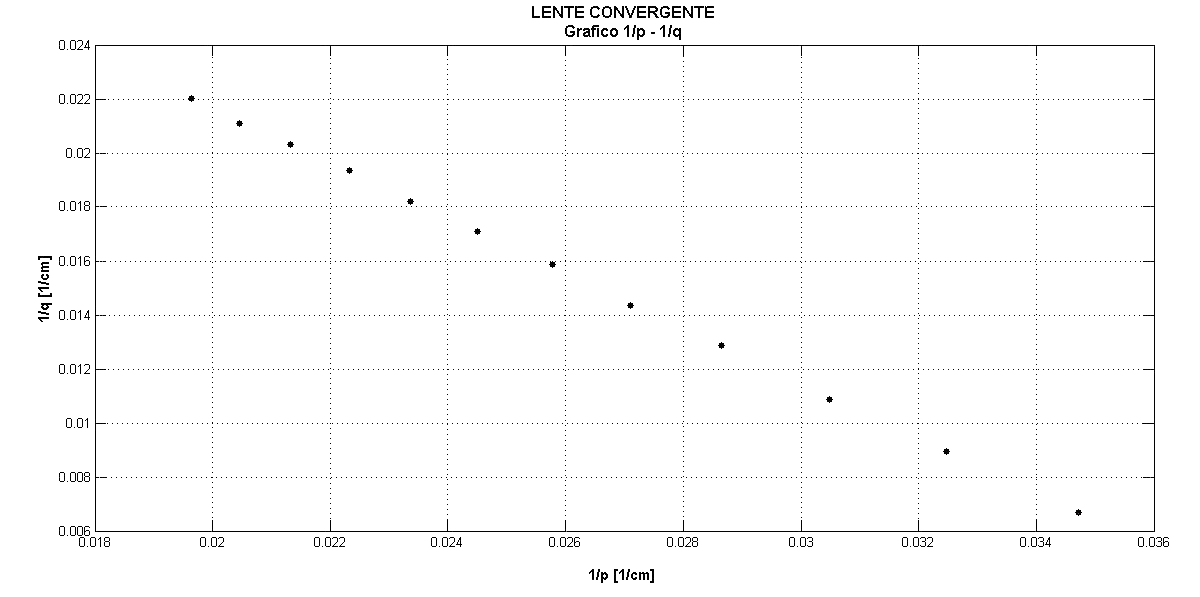
\includegraphics[width=16cm]{grafico_convergente.png}
    \caption{Il grafico mostra la relazione $1/q = - 1/p + 1/f$, che risulta correttamente lineare.}
    \label{fig:graph}
\end{figure}

\subsection{Aberrazione cromatica della lente convergente}

Ogni lente è soggetta a un difetto, detto aberrazione cromatica, dovuto al fatto che l'indice di rifrazione del vetro della lente varia al variare della lunghezza d'onda della luce incidente.
Per valutare e osservare il fenomeno dell'aberrazione cromatica, abbiamo misurato i fuochi della lente convergente per la luce monocromatica rossa e per la luce blu, utilizzando la relazione (\ref{eq:coniugati}).
Per ottenere luce monocromatica abbiamo posto un filtro semitrasparente colorato di fronte alla sorgente luminosa. I valori $p$ e $q$ sono stati presi seguendo lo stesso procedimento adottato per la lente convergente, salvo il fatto che è stato preso solo un valore per ciascuno dei due parametri.

Rosso e blu sono stati scelti per massimizzare la differenza tra i fuochi e facilitare le misure; essi si trovano infatti agli estremi opposti dell'intervallo di lunghezze d'onda della luce visibile e quindi i fuochi sono il più distante possibile tra di loro. Inoltre abbiamo mantenuto $p \simeq q$ per facilitare la misura. Infatti la misura risulta più difficile se $p < q$, come implica la legge dei punti coniugati (\ref{eq:coniugati}), a causa dell'effetto di profondità di campo, e se $p > q$ poiché la distanza tra i fuochi è molto piccola.
I risultati da noi ottenuti sono riportati nella tabella sottostante:
%\begin{SCfigure}
\begin{table}[H]
    \centering
    \small
    \begin{tabular}{l c c c}
        \toprule
		Filtro & $p \; [\si{\centi\metre}]$ & $q \; [\si{\centi\metre}]$ & $f \; [\si{\centi\metre}]$ \\
        \midrule
		Blu & $49.1 \pm 0.1 $ & $46.3 \pm 0.1$ & $24 \pm 2$ \\
		Rosso & $49.1 \pm 0.1$ & $47.4 \pm 0.1$ & $24 \pm 2$ \\
        \bottomrule
    \end{tabular}
    %\caption{voglio il sidecap, damnit!}
    %\label{tab:ab_crom}
\end{table}
%\end{SCfigure}


I fuochi per i due colori risultano compatibili perché l'incertezza è troppo alta per riuscire a distinguere la differenza. Tuttavia, nonostante il valore di $p$ sia costante, $q$ varia, e pure di molto (forse anche troppo, è probabile che una delle misure sia errata), il che ci porta a concludere che siamo riusciti a notare l'effetto dell'aberrazione sferica.

\subsection{Aberrazione sferica della lente convergente}

L'aberrazione sferica è un difetto delle lenti che si verifica quando una lente viene colpita dalla luce in punti lontani dall'asse ottico.
Per osservare il fenomeno dell'aberrazione sferica e valutarne l'importanza, abbiamo misurato il fuoco della lente nel caso in cui la luce incidente fosse:
\begin{itemize}
    \item{un fascio di luce centrale: cioè un insieme di raggi luminosi che investono la lente convergente nel suo centro (raggi parassiali);}
	\item{un fascio di luce divergente: l'insieme dei raggi luminosi che incidono sulla periferia della lente, ovvero sull'anello più distante dal centro;}
\end{itemize}

Abbiamo adottato lo stesso accorgimento del punto precedente, ovvero quello di mantenere $p \simeq p$ al fine di aumentare la differenza tra i fuochi ed evitare una difficile messa a fuoco. Fissata la distanza $p$ abbiamo esaminato il valore di $q$ selezionando prima solo il fascio di luce centrale e poi solo quello periferico. Per selezionari i fasci abbiamo usato un semplice un diaframma; il primo oscurava tutta la superficie a parte una sezione centrale mentre il secondo oscurava tutta la lente a parte un anello circolare vicino al bordo.
I risultati sono riportati nella tabella sottostante:

%\begin{SCfigure}
\begin{table}[H]
    \centering
    \small
    \begin{tabular}{l c c c}
        \toprule
        Diaframma & $p \; [\si{\centi\metre}]$ & $q \; [\si{\centi\metre}]$ & $f \; [\si{\centi\metre}]$ \\
        \midrule
		Foro centrale & p$_b$ & q$_b$ & f$_b$ \\
		Anello periferico & p$_r$ & q$_r$ & f$_r$ \\
        \bottomrule
    \end{tabular}
\end{table}
%\end{SCfigure}


Anche in questo caso l'incertezza sul fuoco non ci permette di distinguere la differenza. Tuttavia, come nel caso precendente il valore $q$ varia e possiamo concludere che abbiamo notato l'effetto dell'aberrazione sferica.

\begin{figure}[h!]
	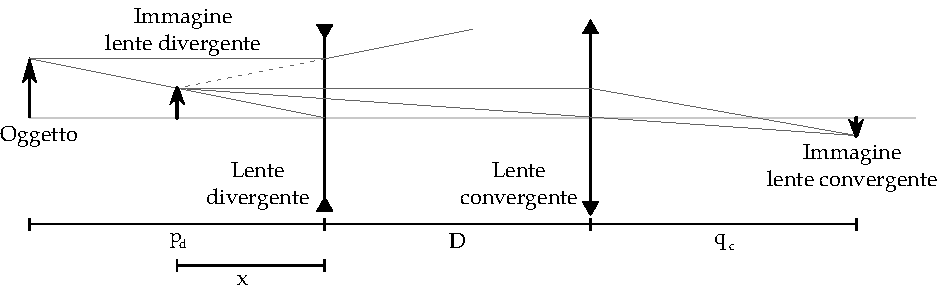
\includegraphics[width=16cm]{drawing2.pdf}
    \caption{Schema della disposizione delle lenti per la misura della focale della lente divergente. È riportata l'immagine
    virtuale della lente divergente e l'immagine finale sullo schermo.}
    \label{fig:div}
\end{figure}

\subsection{Fuoco della lente divergente}

Dal momento che per una lente divergente l'immagine che si ottiene è un immagine virtuale e non reale, ovvero l'immagine non si forma per intersezione dei raggi reali, ma per il loro prolungamento, risulta impossibile mettere a fuoco l'immagine e quindi misurare direttamente il valore di $q$ usando solamente la lente divergente.
Per risolvere il problema abbiamo usato una lente convergente per proiettare l'immagine virtuale su uno schermo (vedi Figura \ref{fig:div}).

%questa non è la figura con le freccette in fondo alla pagina? [STESSA FIGURA PRECEDENTE CON AGGIUNTA LA LENTE DIVERGENTE TRA LA SORGENTE E LA LENTE DIVERGENTE]
% PS che diamine state dicendo? lente Div, tra lente Div e sorgente? quante lenti Div abbiamo? LOL

Specifichiamo da subito la notazione che abbiamo usato (si usi la Figura \ref{fig:div} per riferimento):
\begin{itemize}
	\item{$p\ped{d} = $ distanza tra la sorgente luminosa e il centro della lente divergente;}
	\item{$D = $ distanza tra i centro delle due lenti;}
    \item{$q\ped{c} = $ distanza tra il centro della lente convergente e l'immagine (lo schermo);}
	\item{$x = $ distanza incognita tra il centro della lente divergente e la sua immagine virtuale;}
\end{itemize}

Il sistema di lenti realizzato funziona nel seguente modo: la lente divergente produce un'mmagine virtuale tra la sorgente e se stessa. Qusta immagine diventa quindi il nuovo oggetto per la lente convergente che produce un immagine reale sullo schermo. Quindi potendo misurare tutti i parametri sopraelencati ad eccezione di $x$ e $f\ped{d}$ (focale lente divergente) e conoscendo $f\ped{c}$ (focale lente convergente) si può risolvere il seguente sistema, dato dalla combinazione delle leggi dei punti coniugati per le due lenti:

%\begin{equation}
%	\frac{1}{f\ped{d}} \,=\, \frac{1}{p\ped{d}} + \frac{1}{x}
%	\frac{1}{f\ped{c}} \,=\, \frac{1}{(D + x)} + \frac{1}{q\ped{c}}
%\end{equation}
\begin{equation}
 \left\{
  \begin{aligned}
    \frac{1}{f\ped{d}} & \,=\, \frac{1}{p\ped{d}} + \frac{1}{x}\\
    \frac{1}{f\ped{c}} & \,=\, \frac{1}{(D + x)} + \frac{1}{q\ped{c}}
  \end{aligned}
\right.
\end{equation}

In questo modo si ottengono i valori di $x$ e $f\ped{d}$. Inoltre per ottenere un valore più accurato di $f\ped{d}$, abbiamo eseguito tre misure tenendo ferma la distanza $p\ped{d}$ e variando $D$ e $q\ped{c}$. Quindi per ogni set di misure abbiamo sfruttato la legge dei punti coniugati (\ref{eq:coniugati}) e abbiamo ottenuto tre valori di $f\ped{d}$. Facendone la media si ottiene un valore più accurato di $f\ped{d}$. I risultati sono i seguenti (Il segno negativo indica che l'immagine virtuale ed il fuoco si trovano sul lato sinistro della lente come vista in Figura \ref{fig:div}. Chiaramente esiste anche un altro fuoco dal lato opposto):
\begin{equation}
	x \,=\, (-12 \pm 2) \;\si{\centi\metre} \qquad \qquad f\ped{d} \,=\, (-20 \pm 7) \;\si{\centi\metre}
\end{equation}

Infine anche per questo sistema di lenti abbiamo calcolato il valore della magnificazione nei due modi possibili, cioè indirettamente con i valori $p\ped{d}$, $x$, $D$ e $q\ped{c}$
\begin{equation}
    m\ped{pq} \,=\, m_1 \cdot m_2 \,=\, \frac{x}{p_d} \cdot \frac{q_c}{D+x}
\end{equation} %	|m| \,=\, \frac{x}{p\ped{d}} \,=\,
dove $x$ non è altro che il valore di $q\ped{d}$ e direttamente con i valori di $h$\ped{imm}
\begin{equation}
    m\ped{h} \,=\, \frac{h\ped{imm}}{h}
\end{equation}

\begin{table}[H]
    \centering
    \small
    \begin{tabular}{c c c c c c c c}
        \toprule
        $p_d$ & $x$ & $D$ & $q_c$ & $f_d$ & $m$\ped{ind} & $m$\ped{dir} & $h$\ped{imm} \\
        \midrule
		30.50 $\pm$ 0.05 & -12 $\pm$ 2 & 23.10 $\pm$ 0.05 & 76.00 $\pm$ 0.05 & -20 $\pm$ 6 & 0.9 $\pm$ 0.2 & 0.87 $\pm$ 0.01 & 0.79 $\pm$ 0.01 \\
		30.50 $\pm$ 0.05 & -12 $\pm$ 2 & 25.20 $\pm$ 0.05 & 67.10 $\pm$ 0.05 & -20 $\pm$ 7 & 0.7 $\pm$ 0.2 & 0.71 $\pm$ 0.01 & 0.64 $\pm$ 0.01 \\
		30.50 $\pm$ 0.05 & -12 $\pm$ 3 & 27.20 $\pm$ 0.05 & 61.60 $\pm$ 0.05 & -20 $\pm$ 8 & 0.6 $\pm$ 0.1 & 0.61 $\pm$ 0.01 & 0.55 $\pm$ 0.01 \\
        \bottomrule
    \end{tabular}
    \caption{Commento.}
    \label{tab:div}
\end{table}

%Ovvero conoscendo il valore di $m$ per la lente convergente abbiamo sfruttato la relazione:
%\begin{equation}
%	m \'=\' \frac{h\ped{imm}}{h\ped{ogg}} 
%\end{equation}
%e quindi abbiamo ricavato il valore dell'altezza dell'oggetto per la lente converegente, che però risulta essere nient'altro che l'altezza dell'immagine della lente divergente. Pertanto per ricavare la magnificazione di quest'ultima abbiamo applicato nuovamente la relazione:
%\begin{equation}
%	m \'=\' \frac{h\ped{ogg}}{h} 
%\end{equation}
%e abbiamo ottenuto che $m \'=\' XXX$

\subsection{Indice di rifrazione della lente convergente}

Per ricavare il valore dell'indice di rifrazione $n$ della lente convergente non dobbiamo fare altro che usare la legge del costruttore di lenti:
\begin{equation}
\frac{1}{f} \,=\, (n-1)\left(\frac{1}{R\ped{1}}-\frac{1}{R\ped{2}}\right) \,=\, \frac{2(n-1)}{R}
	\label{eq:costruttore}
\end{equation}
%
\begin{wrapfigure}{r}{20mm}
  \begin{center}
    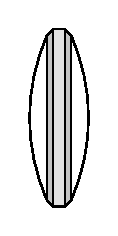
\includegraphics{lente.pdf}
  \end{center}
\end{wrapfigure}
%
dove $f$ è la focale della lente convergente, $R_1$ e $R_2$ sono i raggi delle facce sferiche della lente. La nostra lente era simmetrica per cui $|R_1| = |R_2| \equiv R$ per cui vale la seconda uguaglianza.

Per ottenere il raggio $R$ della lente abbiamo misurato col calibro il diametro della lente, il suo spessore al centro e quello al bordo. Con questi dati ricavare il raggio è un problema di geometria elementare. Tuttavia la nostra lente presentava uno smusso (in figura a lato una sezione), per cui non era chiaro il valore dello spessore al bordo. Abbiamo registrato i valori di spessore al bordo sia includendo lo smusso che non misurandolo. Sono stati ricavati due valori di raggio e dell'indice di rifrazione, in un caso è stata eliminata solo la parte grigio chiaro (senza smusso) mentre nell'altro anche quella grigio scuro (con smusso). I valori ottenuto sono:

\begin{table}[H]
    \centering
    \small
    \begin{tabular}{l c c}
        \toprule
        Smusso & $R \; [\si{\centi\metre}]$ & $n$ \\
        \midrule
		Con smusso & $29 \pm 5$ & $1.6 \pm 0.1$  \\
		Senza smusso & $16 \pm 2$ & $1.3 \pm 0.1$ \\
        \bottomrule
    \end{tabular}
\end{table}







